\documentclass[preprint,12pt,a4paper]{elsarticle}
\usepackage{amssymb}
\usepackage{amsmath}
\usepackage{graphicx}
\usepackage{hyperref}
\usepackage{booktabs}
\usepackage{array}
\usepackage{lineno}
\setlength{\parindent}{0pt}
\setlength{\emergencystretch}{2em}
\newcommand{\gueye}{\texttt{gueye}}
\newcommand{\ii}{\mathrm{i}}
\hypersetup{colorlinks=true,linkcolor=blue,citecolor=blue,urlcolor=blue}
\journal{Mathematics and Computers in Simulation}

\begin{document}
\begin{frontmatter}

\title{\texttt{gueye}: semi-analytic inversion of discrete Laplace/Helmholtz operators in 1D--2D--3D}

\author{Serigne Bira Gueye\corref{cor1}}
\ead{bira.gueye@ucad.edu.sn}
\cortext[cor1]{Corresponding author}
\address{Department of Physics, Faculty of Sciences and Techniques, Cheikh Anta Diop University, Dakar, Senegal}

\begin{abstract}
\texttt{gueye} is a Python package for solving the finite-difference Helmholtz equation on rectangular grids in one, two or three dimensions, with independently specified Dirichlet, Neumann or Robin conditions on each face, and discrete transparent or perfectly matched layer (PML) treatments within their supported directions. It combines a scaled closed-form tridiagonal inverse with transverse diagonalisation. The package computes full fields (including complex prescribed Dirichlet data), selected Green-function values, frequency sweeps and discrete resonances of the full screened operator, and includes a two-dimensional Dirichlet obstacle and time-domain responses. Validation against independent dense, sparse and explicit-layer references shows near-roundoff agreement for tested discrete problems and second-order convergence against continuous solutions.
\end{abstract}

\begin{keyword}
Helmholtz equation \sep finite differences \sep tridiagonal matrix inverse \sep Green function \sep perfectly matched layer \sep Python
\end{keyword}

\end{frontmatter}

\linenumbers

\section{Motivation and significance}
Finite-difference discretisations of the Poisson and Helmholtz equations give Kronecker-sum matrices whose one-dimensional factors are tridiagonal.
Fast direct solvers exploit this: tensor-product methods~\cite{LynchRiceThomas1964}, Fourier-based methods and cyclic reduction~\cite{Hockney1965,BuzbeeGolubNielson1970}.
Specialised transforms are highly efficient for regular operators and compatible boundary conditions; a sine transform, for instance, assumes Dirichlet data on every face.
Practitioners who change the boundary condition on each face, the frequency, or the receiver positions need a framework in which these are parameters, and who often want a handful of field values rather than a whole grid.

The inverse of a tridiagonal matrix has a closed form in terms of two sequences of minors~\cite{Usmani1994,HuOConnell1996,DaFonsecaPetronilho2001}, reviewed in~\cite{Meurant1992}.
The author used it for the 1D Poisson and Helmholtz equations~\cite{Gueye2014a,Gueye2014b,Gueye2014c,Gueye2014d} and for the 2D Poisson equation through the pentadiagonal Laplacian~\cite{Gueye2022}; a general second-order BTCS+CTCS scheme using Usmani's inversion is in~\cite{Gueye2021}.
\gueye{} is a reusable implementation that (i) evaluates the closed form safely for complex and non-symmetric coefficients and free end rows, (ii) reaches 2D and 3D by transverse diagonalisation, as in classical separation of variables~\cite{LynchRiceThomas1964}, with arbitrary end conditions on the remaining axis, (iii) includes exact discrete transparent and PML conditions, and (iv) provides pointwise Green values, sweeps, safeguards and a time-domain layer.

\section{Software description}
\subsection{Software architecture}
\paragraph{Kernel.}
For a tridiagonal $T$ with sub-, main and super-diagonal $l,d,u$ and roots $r_{1,2}$ of $x^2-dx+lu=0$,
\begin{equation}\label{eq:usmani}
(T^{-1})_{ij}=(-1)^{i+j}\,u^{\,j-i}\,\frac{\theta_{i-1}\,\varphi_{j+1}}{\theta_N}\quad(i\le j),\qquad
\theta_i=\frac{r_1^{\,i+1}-r_2^{\,i+1}}{r_1-r_2},
\end{equation}
with $\theta_i$, $\varphi_i$ the leading and trailing minors~\cite{Usmani1994}.
\texttt{TridiagInverse} evaluates~\eqref{eq:usmani} with scaled variables (hyperbolic, oscillatory and double-root regimes) and supports Neumann or Robin end rows (real or complex $\alpha$) through a ghost node.
A solve costs $O(N)$, a single entry $O(1)$ after set-up, and a LAPACK \texttt{gttrf} factorisation is cached for repeated right-hand sides.
A relative-determinant check raises \texttt{SingularOperator} below $10^{-10}$ and warns below $10^{-6}$.

\paragraph{2D and 3D.}
In 2D, $T_x=V\Lambda V^{-1}$ is diagonalised (\texttt{eigh\_tridiagonal} if symmetric, \texttt{eig} otherwise) and each mode $\nu$ gives a tridiagonal system in $y$ with shift $\lambda_\nu$, solved with the kernel.
In 3D, $x$ and $y$ are diagonalised and $z$ stays in closed form with the shift $\lambda^x_\nu+\lambda^y_{\nu'}$.
Since all modes share the same $N$, class \texttt{ModeStack} runs one vectorised $O(N)$ sweep over all modes instead of a Python loop of LU solves.
For a fixed grid, the modal solve scales with the number of unknowns ($O(N_xN_y)$ in 2D and $O(N_xN_yN_z)$ in 3D); the full multidimensional inverse is never formed. Symmetric transverse tridiagonal operators use a dedicated tridiagonal eigensolver, whereas nonsymmetric transverse operators use a general eigensolver, whose set-up cost can dominate for large transverse dimensions. The modal arrays and transformed field require storage proportional to the grid size.

\paragraph{Open boundaries.}
The exact transparent condition (\texttt{"A"}, last axis) is the Schur complement of the discrete half-space, a geometric sequence of ratio $r$.
A PML of $m$ cells with stretching $s(t)=1-\ii\sigma(t)/k$, $\sigma(t)=\sigma_{\max}(t/\delta)^p$, $\sigma_{\max}=(p+1)\ln(1/R_0)/(2\delta)$~\cite{Berenger1994} is eliminated by a backward Schur recurrence into the end row of the closed axis; on diagonalised axes the layer nodes are explicit and re-diagonalised per frequency.

\subsection{Software functionalities}
The interface \texttt{gy.problem(size, cells, bc, k, mu)} takes one pair of conditions per axis; prescribed Dirichlet values may be complex constants or coordinate-dependent functions, \texttt{"D"}, \texttt{("N",g)}, \texttt{("R",alpha,g)}, \texttt{"A"}, and \texttt{("P",m,R0)}, and provides
\texttt{solve} (full field), \texttt{green} and \texttt{at} (point values), \texttt{sweep} (frequency response, \texttt{NaN} at singular frequencies), \texttt{resonances} (eigen-wavenumbers of $-\Delta_h+\mu^2$, with $k_n^2=\lambda_n+\mu^2$; complex $k$ when the spectrum is not real positive), and \texttt{with\_k}.
Sources on Dirichlet nodes and points outside the box raise \texttt{ValueError}.
\path{recipes.dirichlet_obstacle} treats a 2D Dirichlet obstacle by a capacitance matrix.
The wave equation is advanced by the Newmark scheme ($\beta=1/4$, $\gamma=1/2$) with a matrix inverted once; boundary data $g_0(\mathbf x)s(t)$ may depend on time (\texttt{bc\_time}), and \path{recipes.time_response} gives open-domain responses (PML or transparent) by Fourier synthesis over complex frequencies; the PML is not available step by step.

\paragraph{Interactive graphical interface (version 0.7.2).}
The package now includes an optional browser-based interface launched with \texttt{gueye-gui} or \texttt{python -m gueye.gui}. It is implemented with Python's standard-library HTTP server and an embedded HTML/JavaScript page, so it adds no mandatory GUI framework. The interface supports exploratory field visualization in 1D--3D, face-by-face boundary-condition selection, source and receiver placement, frequency sweeps, discrete-resonance display, a two-dimensional circular obstacle, and time-domain wave animation. Calculations call the package API; the interface is intended for local exploration and visualization, not as a network service or as independent validation of the numerical methods. The server binds to the loopback interface, checks local Host/Origin authorities against the loopback server and its port, and applies request-size and grid-size limits.

\section{Illustrative examples}
\paragraph{Open-domain scattering.}
Figure~\ref{fig:open} shows a point source scattered by a Dirichlet disc in a domain open on all four faces (PML, $m=16$, $R_0=10^{-8}$, $k=16$, grid $200\times150$ on $4\times3$), from \path{examples/ex5_ouvert_complet.py}.
\begin{figure}[t]
\centering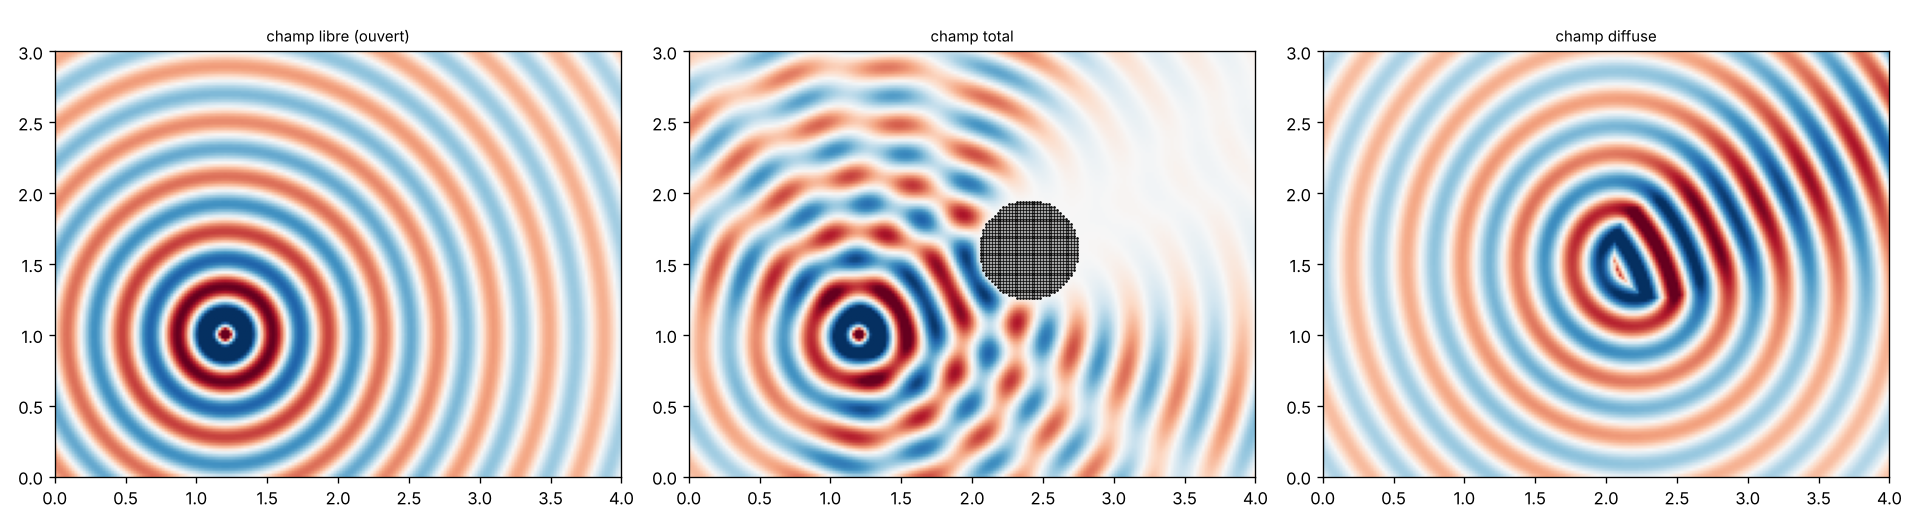
\includegraphics[width=\textwidth]{../examples/ex5_ouvert_complet.png}
\caption{Free, total and scattered fields (real part) for a point source and a Dirichlet disc in a domain with PML on four faces.}\label{fig:open}
\end{figure}

\paragraph{Interactive exploration.}
Figure~\ref{fig:gui} shows the interactive field view for a point source in a two-dimensional domain containing a circular Dirichlet obstacle. The visualization illustrates the spatial field pattern and obstacle placement; it is an interface example rather than a separate numerical validation result.
\begin{figure}[t]
\centering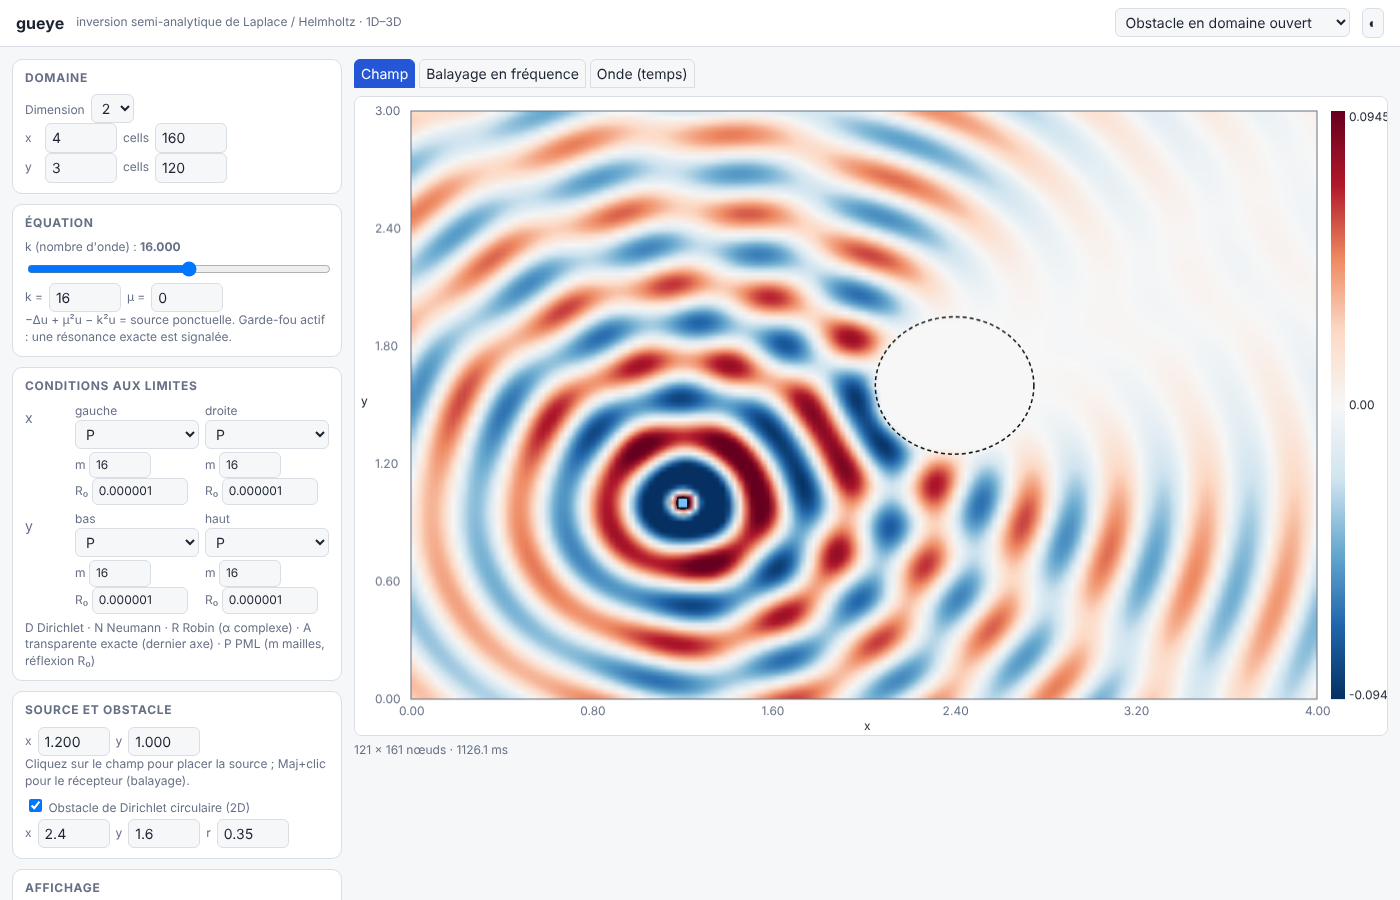
\includegraphics[width=\textwidth]{../examples/gui_open_obstacle.png}
\caption{Interactive field visualization for a point source and a circular Dirichlet obstacle in a two-dimensional domain. The colour scale represents the real-valued field; the dashed circle marks the obstacle.}
\label{fig:gui}
\end{figure}

\paragraph{Validation.}
Table~\ref{tab:valid} lists comparisons with independent references; the repository contains the scripts (\texttt{validation/}) and 166 automated tests.
\begin{table}[t]
\centering\small
\begin{tabular}{@{}p{5.0cm}p{3.5cm}p{3.5cm}@{}}
\toprule
Check & Independent reference & Observed result\\
\midrule
1D kernel, 89 cases & Dense inverse & $2.64\times10^{-7}$ worst case, near singularity; typically $10^{-14}$--$10^{-12}$\\
2D modal solve, 12 boundary configurations & Sparse direct solve & $2.8\times10^{-13}$ maximum\\
3D modal solve, 8 boundary configurations & Sparse direct solve & $1.5\times10^{-14}$ maximum\\
Continuous-solution convergence & Manufactured solutions, 1D--3D & Order $2.00$ in 1D/2D; $1.99$--$2.00$ in 3D\\
PML elimination, 1D & Explicit layer matrix & $7.3\times10^{-14}$\\
Newmark, 2D and 3D & Sparse LU time stepping & $9.2\times10^{-15}$ and $3.4\times10^{-15}$\\
\bottomrule
\end{tabular}
\caption{Validation results from the included scripts and regression tests. Errors are maximum relative deviations unless otherwise indicated. The boundary-condition configurations are representative, not an exhaustive enumeration of all possible face combinations.}
\label{tab:valid}
\end{table}
\paragraph{Independent reference checks.}
A dedicated script, \texttt{validation/test\_independent\_references.py}, compares the package against independently assembled sparse systems. Green-function columns are checked against sparse direct solutions with a point source scaled by the cell volume; frequency sweeps are checked at three complex wavenumbers against three separate sparse solves; discrete resonances are checked against the eigenvalues of the assembled discrete operator. Table~\ref{tab:independent} reports the maximum relative deviations.
\begin{table}[t]
\centering\small
\begin{tabular}{@{}lrrr@{}}
\toprule
Dimension & Green column & Frequency sweep & Discrete resonances\\
\midrule
1D & $2.42\times10^{-14}$ & $3.28\times10^{-14}$ & $5.33\times10^{-15}$\\
2D & $1.45\times10^{-14}$ & $1.02\times10^{-14}$ & $3.51\times10^{-15}$\\
3D & $9.88\times10^{-16}$ & $6.44\times10^{-16}$ & $2.38\times10^{-15}$\\
\bottomrule
\end{tabular}
\caption{Independent sparse-reference checks for Green columns, three-frequency sweeps, and discrete resonance wavenumbers.}
\label{tab:independent}
\end{table}
\paragraph{Dirichlet obstacles.}
The embedded-obstacle capacitance formulation was compared with a direct sparse solve in which obstacle nodes are eliminated from the matrix. For circular and rectangular obstacles on $64\times32$ and $128\times64$ grids, the maximum relative field deviation was $1.58\times10^{-14}$; the maximum residual field on obstacle nodes was $7.22\times10^{-16}$. These are discrete-algebraic comparisons, not a validation of arbitrary curved-boundary geometries or of a continuum obstacle model.
\paragraph{Residual PML reflection.}
The algebraic elimination of the explicit PML layer agrees with the reduced system to $7.3\times10^{-14}$ in the reproducible 1D explicit-layer comparison. This algebraic check is distinct from physical absorption: relative field deviations against the discrete transparent reference were $3.8\times10^{-6}$ for a 1D layer with $m=32$, $R_0=10^{-6}$ and $kh=0.2$; in 2D, with $m=16$ and $R_0=10^{-6}$, they ranged from $1.6\times10^{-5}$ to $2.3\times10^{-3}$ over tested modal incidence angles $4^\circ$--$64^\circ$; in 3D, a $12$-cell layer gave $4.3\times10^{-3}$. These errors depend on layer thickness, target reflection parameter and incidence angle for the tested configurations; they are field deviations, not reflection coefficients. A broad frequency-dependent PML parameter study remains future work.
\paragraph{Time-domain open-boundary check.}
For the 1D open-domain response, Fourier synthesis with the exact discrete transparent condition differed from a large-domain Newmark reference by $1.7\times10^{-3}$ in maximum amplitude-normalised error. A PML with $m=24$ and $R_0=10^{-10}$ gave $2.7\times10^{-3}$. The time-domain PML is implemented through frequency synthesis; step-by-step Newmark propagation with a PML is not claimed.
The corrective release test run used Python 3.13.5, NumPy 2.3.5 and SciPy 1.17.0; all 166 tests passed. The GitHub Actions test and installation-smoke-test matrix passed on Python 3.9, 3.10, 3.11, 3.12 and 3.13 on both Ubuntu 24.04 and Windows Server 2022. macOS was not validated. These timings describe the local test environment and are not performance guarantees.

\section{Performance}
A separate reproducible benchmark script, \path{validation/benchmark_reproducible.py}, separates modal setup, modal solve, sparse matrix assembly, sparse LU factorisation, and sparse triangular solves. It reports medians over repeated measurements and writes the raw results to CSV. The following measurements cover homogeneous Dirichlet and mixed Dirichlet--Neumann configurations on Linux with Python 3.13.5, NumPy 2.3.5 and SciPy 1.17.0 (five repetitions; one right-hand side unless noted).

\begin{table}[t]
\centering\small
\resizebox{\textwidth}{!}{%
\begin{tabular}{@{}p{2.5cm}rrrrr@{}}
\toprule
Case & Unknowns & \shortstack{Modal setup\\(ms)} & \shortstack{Modal solve\\(ms)} & \shortstack{Sparse factor\\(ms)} & \shortstack{Sparse solve\\(ms)}\\
\midrule
2D, DDDD, $40\times32$ & 1,209 & 1.95 & 0.277 & 1.73 & 0.0610\\
2D, DN/ND, $40\times32$ & 1,280 & 1.83 & 0.251 & 1.86 & 0.0613\\
3D, DDDDDD, $12\times10\times8$ & 693 & 3.94 & 0.351 & 2.05 & 0.0489\\
3D, DN/ND/DN, $12\times10\times8$ & 960 & 4.56 & 0.301 & 3.47 & 0.0761\\
\bottomrule
\end{tabular}}
\caption{Five-repeat benchmark. Sparse assembly times were 0.98, 0.66, 1.28 and 1.42 ms in row order; four right-hand sides took 0.131, 0.153, 0.123 and 0.185 ms. Relative differences from the sparse direct solutions were $5.8\times10^{-15}$, $4.2\times10^{-14}$, $1.3\times10^{-15}$ and $7.2\times10^{-15}$.}
\label{tab:bench}
\end{table}

These are small representative problems and show that sparse direct solves can be faster for a single right-hand side at these sizes. The benchmark is intended to make the comparison reproducible, not to claim universal speed superiority. The method's value is its combination of face-by-face boundary conditions, pointwise Green values, frequency sweeps, and the closed-form axis solve. For a cube with homogeneous Dirichlet data, a discrete sine transform remains the natural specialised comparator.

\section{Impact}
\gueye{} lets a user change boundary conditions face by face, obtain Green values or frequency responses, and locate resonances of the discrete operator without assembling or factorising a sparse matrix for each case, and with guards against silent failures near resonances.
It supports teaching and verification of finite-difference codes, since solutions are exact for the discrete operator up to rounding.
\emph{Limitations:} the exact transparent condition applies to the last axis only; the PML is exact algebraically but keeps a configuration-dependent residual field error ($3.8\times10^{-6}$--$10^{-2}$ in our tests); a frequency sweep with a PML on a diagonalised axis re-diagonalises per frequency; Newmark has no step-by-step PML; first-order terms are 1D only; the domain is a rectangular box, with a 2D embedded obstacle; the scheme is second order, with grid dispersion of order $(kh)^2/24$.

\section{Conclusions}
\gueye{} combines a safe closed-form tridiagonal inverse with transverse diagonalisation to treat mixed, transparent and PML conditions in one to three dimensions, with documented accuracy and limits.
Future work includes the general BTCS+CTCS scheme of~\cite{Gueye2021}, step-by-step PML, and 3D obstacles.

\section*{Acknowledgements}
This research did not receive any specific grant from funding agencies in the public, commercial, or not-for-profit sectors.

\section*{Funding}
This research did not receive any specific grant from funding agencies in the public, commercial, or not-for-profit sectors.

\section*{Declaration of competing interests}
The author declares no known competing financial interests or personal relationships that could have appeared to influence the work reported in this paper.

\section*{CRediT authorship contribution statement}
Serigne Bira Gueye: Conceptualization, Methodology, Software, Validation, Investigation, Writing -- original draft, Writing -- review and editing.

\section*{Data availability}
No separate research dataset was generated for this software description. The source archive, examples, and validation scripts accompany the release package. The public source repository and the corrected source branch are available at \url{https://github.com/sbirag/gueye/tree/release/0.7.2}; a tagged 0.7.2 release and a permanent archive identifier (for example, a Zenodo DOI) remain to be created before final submission.

\section*{Declaration of generative AI and AI-assisted technologies in the manuscript preparation process}
During software development and the preparation of this manuscript, the author used ChatGPT (OpenAI) and Claude (Anthropic) for assistance with drafting and editing, code review and verification, troubleshooting, and technical advice. The author reviewed the suggestions and remains responsible for the software, the verification and interpretation of numerical results, the scientific content, and the final manuscript. The AI tools are not authors and were not treated as substitutes for executing the software tests or independently assessing the reported results.

\begin{thebibliography}{99}
\bibitem{LynchRiceThomas1964} R.~E. Lynch, J.~R. Rice, D.~H. Thomas, Direct solution of partial difference equations by tensor product methods, Numer.\ Math.\ 6 (1964) 185--199.
\bibitem{Hockney1965} R.~W. Hockney, A fast direct solution of Poisson's equation using Fourier analysis, J.\ ACM 12 (1965) 95--113.
\bibitem{BuzbeeGolubNielson1970} B.~L. Buzbee, G.~H. Golub, C.~W. Nielson, On direct methods for solving Poisson's equations, SIAM J.\ Numer.\ Anal.\ 7 (1970) 627--656.
\bibitem{Usmani1994} R.~A. Usmani, Inversion of a tridiagonal Jacobi matrix, Linear Algebra Appl.\ 212--213 (1994) 413--414. \url{https://doi.org/10.1016/0024-3795(94)90414-6}
\bibitem{HuOConnell1996} G.~Y. Hu, R.~F. O'Connell, Analytical inversion of symmetric tridiagonal matrices, J.\ Phys.\ A 29 (1996) 1511--1513. \url{https://doi.org/10.1088/0305-4470/29/7/020}
\bibitem{DaFonsecaPetronilho2001} C.~M. da Fonseca, J.~Petronilho, Explicit inverses of some tridiagonal matrices, Linear Algebra Appl.\ 325 (2001) 7--21. \url{https://doi.org/10.1016/S0024-3795(00)00289-5}
\bibitem{Meurant1992} G.~Meurant, A review on the inverse of symmetric tridiagonal and block tridiagonal matrices, SIAM J.\ Matrix Anal.\ Appl.\ 13 (1992) 707--728.
\bibitem{Berenger1994} J.-P. B\'erenger, A perfectly matched layer for the absorption of electromagnetic waves, J.\ Comput.\ Phys.\ 114 (1994) 185--200.
\bibitem{Gueye2014a} S.~B. Gueye, The exact formulation of the inverse of the tridiagonal matrix for solving the 1D Poisson equation with the finite difference method, J.\ Electromagn.\ Anal.\ Appl.\ 6 (2014) 303--308. \url{https://doi.org/10.4236/jemaa.2014.610030}
\bibitem{Gueye2014b} S.~B. Gueye, K.~Talla, C.~Mbow, Solution of 1D Poisson equation with Neumann--Dirichlet and Dirichlet--Neumann boundary conditions, using the finite difference method, J.\ Electromagn.\ Anal.\ Appl.\ 6 (2014) 309--318. \url{https://doi.org/10.4236/jemaa.2014.610031}
\bibitem{Gueye2014c} S.~B. Gueye, K.~Talla, C.~Mbow, Generalization of the exact solution of 1D Poisson equation with Robin boundary conditions, using the finite difference method, J.\ Electromagn.\ Anal.\ Appl.\ 6 (2014) 372--381. \url{https://doi.org/10.4236/jemaa.2014.612038}
\bibitem{Gueye2014d} S.~B. Gueye, Semi-analytical solution of the 1D Helmholtz equation, obtained from inversion of symmetric tridiagonal matrix, J.\ Electromagn.\ Anal.\ Appl.\ 6 (2014) 425--438. \url{https://doi.org/10.4236/jemaa.2014.614044}
\bibitem{Gueye2021} S.~B. Gueye, C.~Mbow, M.~F. Diagana, Efficient BTCS + CTCS finite difference scheme for general linear second order PDE, J.\ Electromagn.\ Anal.\ Appl.\ 13 (2021) 135--143. \url{https://doi.org/10.4236/jemaa.2021.1310010}
\bibitem{Gueye2022} S.~B. Gueye, Exact inversion of pentadiagonal matrix for semi-analytic solution of 2D Poisson equation, J.\ Mod.\ Phys.\ 13 (2022) 1525--1529. \url{https://doi.org/10.4236/jmp.2022.1312094}
\end{thebibliography}

\section*{Software availability}
The software described in this article is \texttt{gueye} version 0.7.2, distributed under the MIT License. The source code, tests, examples and validation scripts are available in the public repository at \url{https://github.com/sbirag/gueye/tree/release/0.7.2}. The release branch was tested by GitHub Actions on Python 3.9--3.13 on Ubuntu 24.04 and Windows Server 2022. A tagged release and a permanent archival DOI have not yet been created; these will be added only after the final author-approved source freeze.

\end{document}
\endinput
